\documentclass{article}
\usepackage[utf8]{inputenc}
\usepackage{amsmath}
\usepackage{graphicx}
\usepackage[a4paper, total={6in, 10in}]{geometry}
\usepackage{float}
\usepackage{caption}
\usepackage{hyperref}
\usepackage{subcaption}
\newcommand{\xdashrightarrow}[2][]{\ext@arrow 0359\rightarrowfill@@{#1}{#2}}

\title{Big data 1}
\author{Anton Rosenberg}
\date{May 2022}

\begin{document}

\maketitle
\newpage
\section{a}
\subsection{Results}
The three classifiers i choose to implement were Random forest, SVM and Logistic regression. Using these three methods stratisfied K fold was used with 5 folds and the scores of the models were averaged over the folds. Furthermore the entire process was run 100 times and the final scores were the mean of the scores during these runs see table \ref{score}. The only data prepossessing made was to normalise the data so that all features have values between 0 and 1.
\begin{table}[H]
    \centering
    \begin{tabular}{c|c|c|c|c}
        Model & accuracy & std & TPR & TNR \\
         SVM & 0.814 & 0.056 & 0.818 & 0.808 \\
         Random forest & 0.75 & 0.065 & 0.781 & 0.714 \\
         Logistic regression & 0.762 & 0.057 & 0.743 & 0.783
    \end{tabular}
    \caption{Scores for the different models}
    \label{score}
\end{table}
Finally a record of the images which were classified incorrectly was kept during the 100 runs and can be seen in figure \ref{wrong}, here the x-axis represents the picture number and the y-axis the number of times that picture was incorrectly classified.
\begin{figure}[ht]
\begin{subfigure}{.33\textwidth}
  \centering
  % include first image
  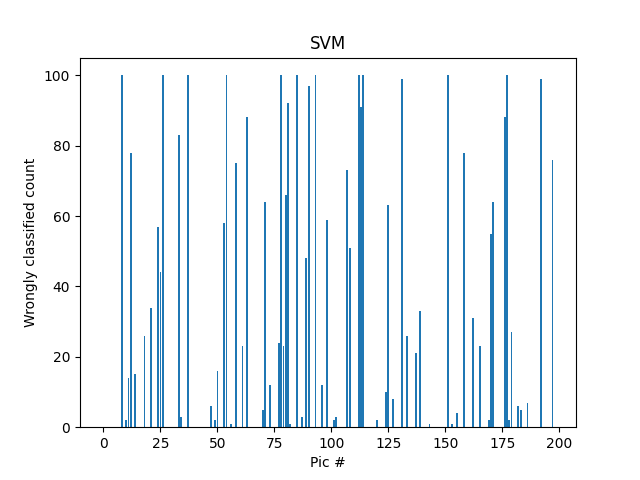
\includegraphics[width=1\linewidth]{1a/SVM.png}  
  \caption{Put your sub-caption here}
  \label{fig:sub-first}
\end{subfigure}
\begin{subfigure}{.33\textwidth}
  \centering
  % include second image
  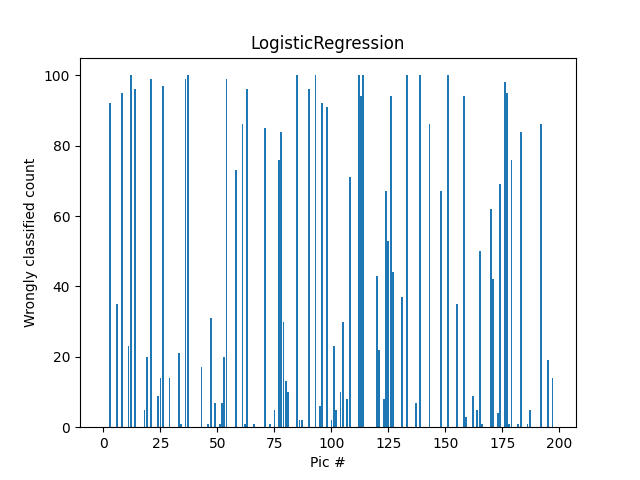
\includegraphics[width=1\linewidth]{1a/Logistic regression.png}  
  \caption{Put your sub-caption here}
  \label{fig:sub-second}
\end{subfigure}
\begin{subfigure}{.33\textwidth}
  \centering
  % include second image
  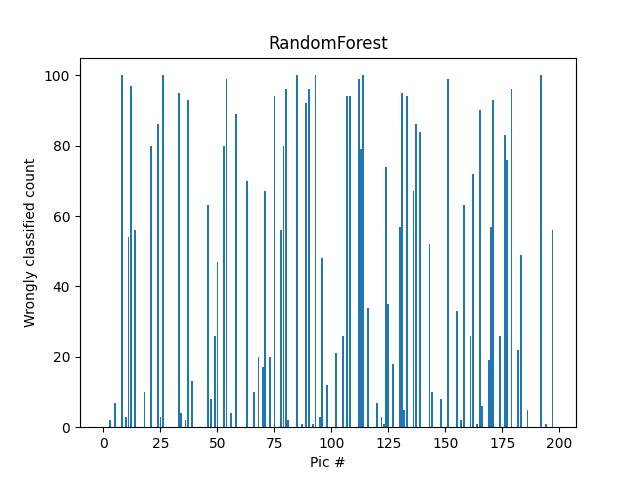
\includegraphics[width=1\linewidth]{1a/Random Forest.png}  
  \caption{Put your sub-caption here}
  \label{fig:sub-second}
\end{subfigure}
\caption{Put your caption here}
\label{wrong}
\end{figure}
\subsection{Discussion}
From the scores we can see that the SVM model preforms better than the others this could be due to the fact that SVM works well when we don't know alot about the data and how it's distributed which is the case for the images in the CATSnDOGS data set. Moreover SVM is less prone to overfiting due to it being a maximum margin classifier which could be an explanation for why it has a higher accuracy than the other models. Its suprising that the logistic regression model worked so well since we have alot less samples than features and we haven't done any feature reduction. This could be due to the fact that the l2 penalisation was used to minimize the negative effect of having less samples than features. When looking at the difference between classifying dogs and cats we look at the TPR which is the rate at which dogs are correctly classified and the TNR the same for the cats. We can see that the models have roughly the same amount of errors for both the dogs and the cats which would indicate that they are equaly difficult to predict. When looking at the images which were consistenly mislabeled there were a few which pictures which were incorrectly classified all the time by all classifiers. One example of these pictures can be seen in \ref{faulty data}. Here we see that the image clearly is of a cat but the label says it's a dog so we have some incorrectly labeled pictures in our data set which explains why they are incorrectly classified. There are probably some pictures which are outliers aswell which would make them difficult to classify correctly for example a dog with very catlike features. 
\begin{figure}[H]
    \centering
    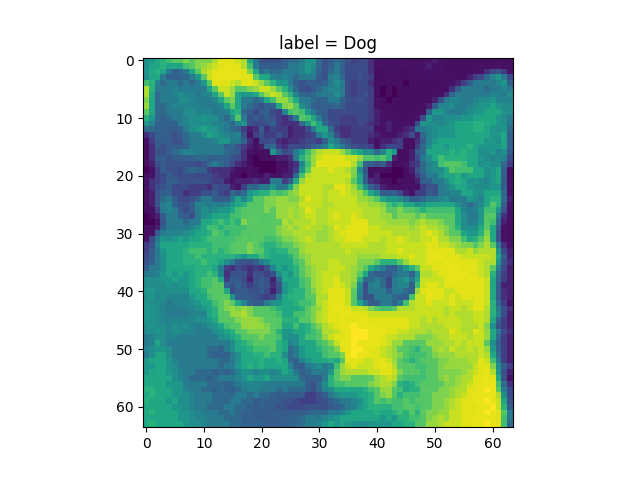
\includegraphics[scale=0.5]{1a/Dirty data.png}
    \caption{Faulty data}
    \label{faulty data}
\end{figure}
\newpage
\section{b}
\subsection{Result}
The three different methods used for finding the most important features were, select K best with chi2 score, variance filtering and linearSVC. Bootstrapping was used 100 times to see which features were selected with high certainty the results for each method can be seen in figure \ref{imp feat} and figure \ref{imp pixels}. 
\begin{figure}[ht]
\begin{subfigure}{.33\textwidth}
  \centering
  % include first image
  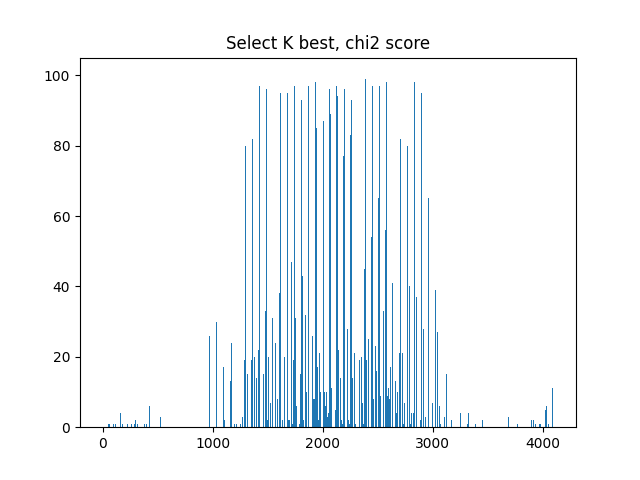
\includegraphics[width=1\linewidth]{1b/Figure_2.png}  
  \caption{Put your sub-caption here}
  \label{fig:sub-first}
\end{subfigure}
\begin{subfigure}{.33\textwidth}
  \centering
  % include second image
  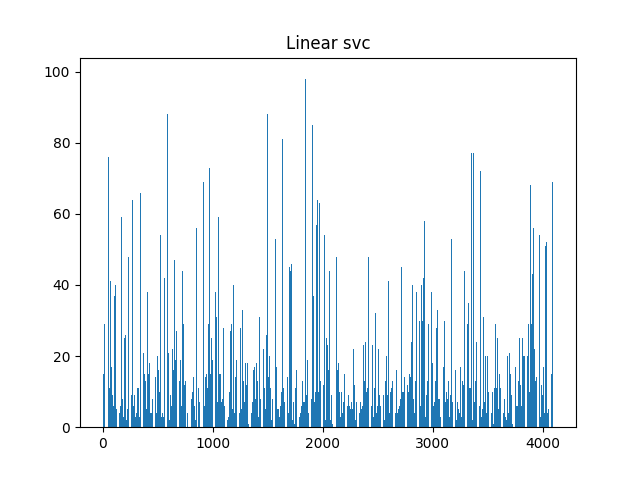
\includegraphics[width=1\linewidth]{1b/Figure_3.png}  
  \caption{Put your sub-caption here}
  \label{fig:sub-second}
\end{subfigure}
\begin{subfigure}{.33\textwidth}
  \centering
  % include second image
  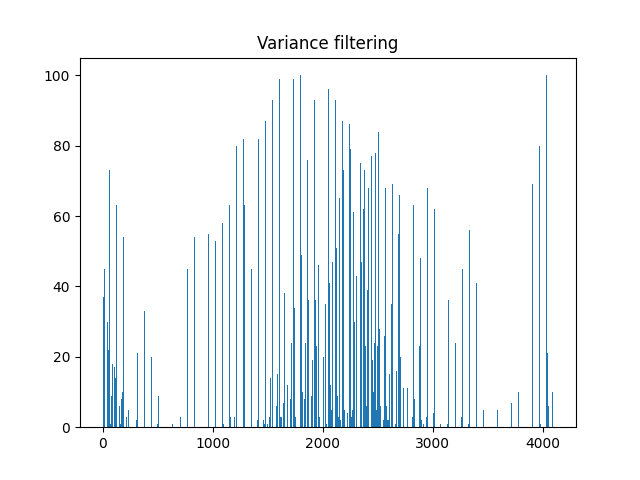
\includegraphics[width=1\linewidth]{1b/Figure_1.png}  
  \caption{Put your sub-caption here}
  \label{fig:sub-second}
\end{subfigure}
\caption{Put your caption here}
\label{imp feat}
\end{figure}

\begin{figure}[ht]
\begin{subfigure}{.33\textwidth}
  \centering
  % include first image
  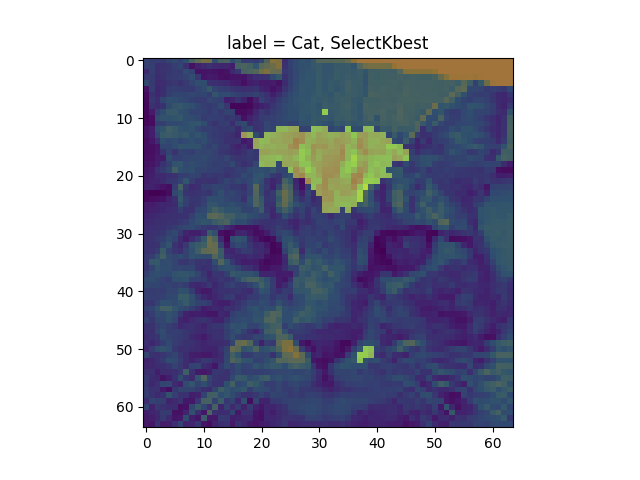
\includegraphics[width=1\linewidth]{1b/Imp_feat_kbest.png}  
  \caption{Put your sub-caption here}
  \label{fig:sub-first}
\end{subfigure}
\begin{subfigure}{.33\textwidth}
  \centering
  % include second image
  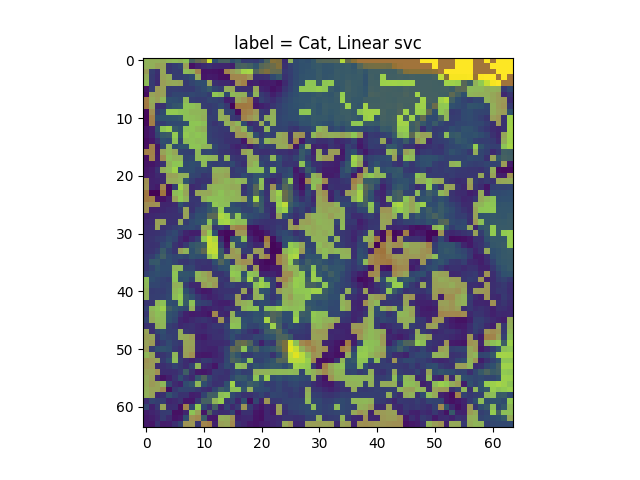
\includegraphics[width=1\linewidth]{1b/Imp_feat_svc.png}  
  \caption{Put your sub-caption here}
  \label{fig:sub-second}
\end{subfigure}
\begin{subfigure}{.33\textwidth}
  \centering
  % include second image
  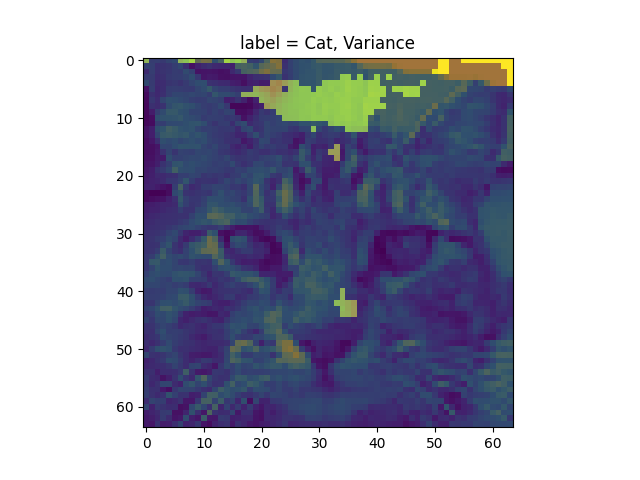
\includegraphics[width=1\linewidth]{1b/Imp_feat_var.png}  
  \caption{Put your sub-caption here}
  \label{fig:sub-second}
\end{subfigure}
\caption{Put your caption here}
\label{imp pixels}
\end{figure}
\subsection{Discussion}
We can see that both select K best and variance filtering seem to look mostly at pixels around the ears area which makes sense since the ears between cats and dogs are generally very different. There is however some difference between the select Kbest and variance filtering even though they have some overlap and seem to both be looking primarily at the ears. As for the linear SVC method it's difficult to see why these pixels are deemed important since they don't cluster around any given area of the picture like the around the eyes for example. This could be because the linear kernal is poorly suited for this data set this could also be why so few pixels were selected above the threshold of 80\%.  The stability of the chosen pixels is improved vastly by bootstrapping and choosing a threshold were only features selected more than the threshold are kept. The threshold was set at 80\% for the pixels shown in \ref{imp pixels}. 
\newpage
\section{c}
\subsection{Result}
The clustering method used was gaussian mixture model and the data was preprocessed by normalization and using principle components. A cutoff at 0.03 was chosen to decide the numbber of PCA used (5) when transforming the data see figure \ref{scree}.  
\begin{figure}[H]
    \centering
    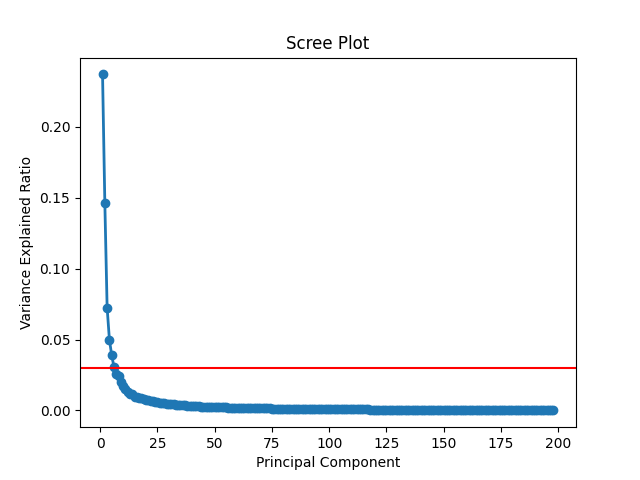
\includegraphics[scale=0.4]{1c/Scree plot.png}
    \caption{Caption}
    \label{scree}
\end{figure}
\begin{figure}[ht]
\begin{subfigure}{.5\textwidth}
  \centering
  % include first image
  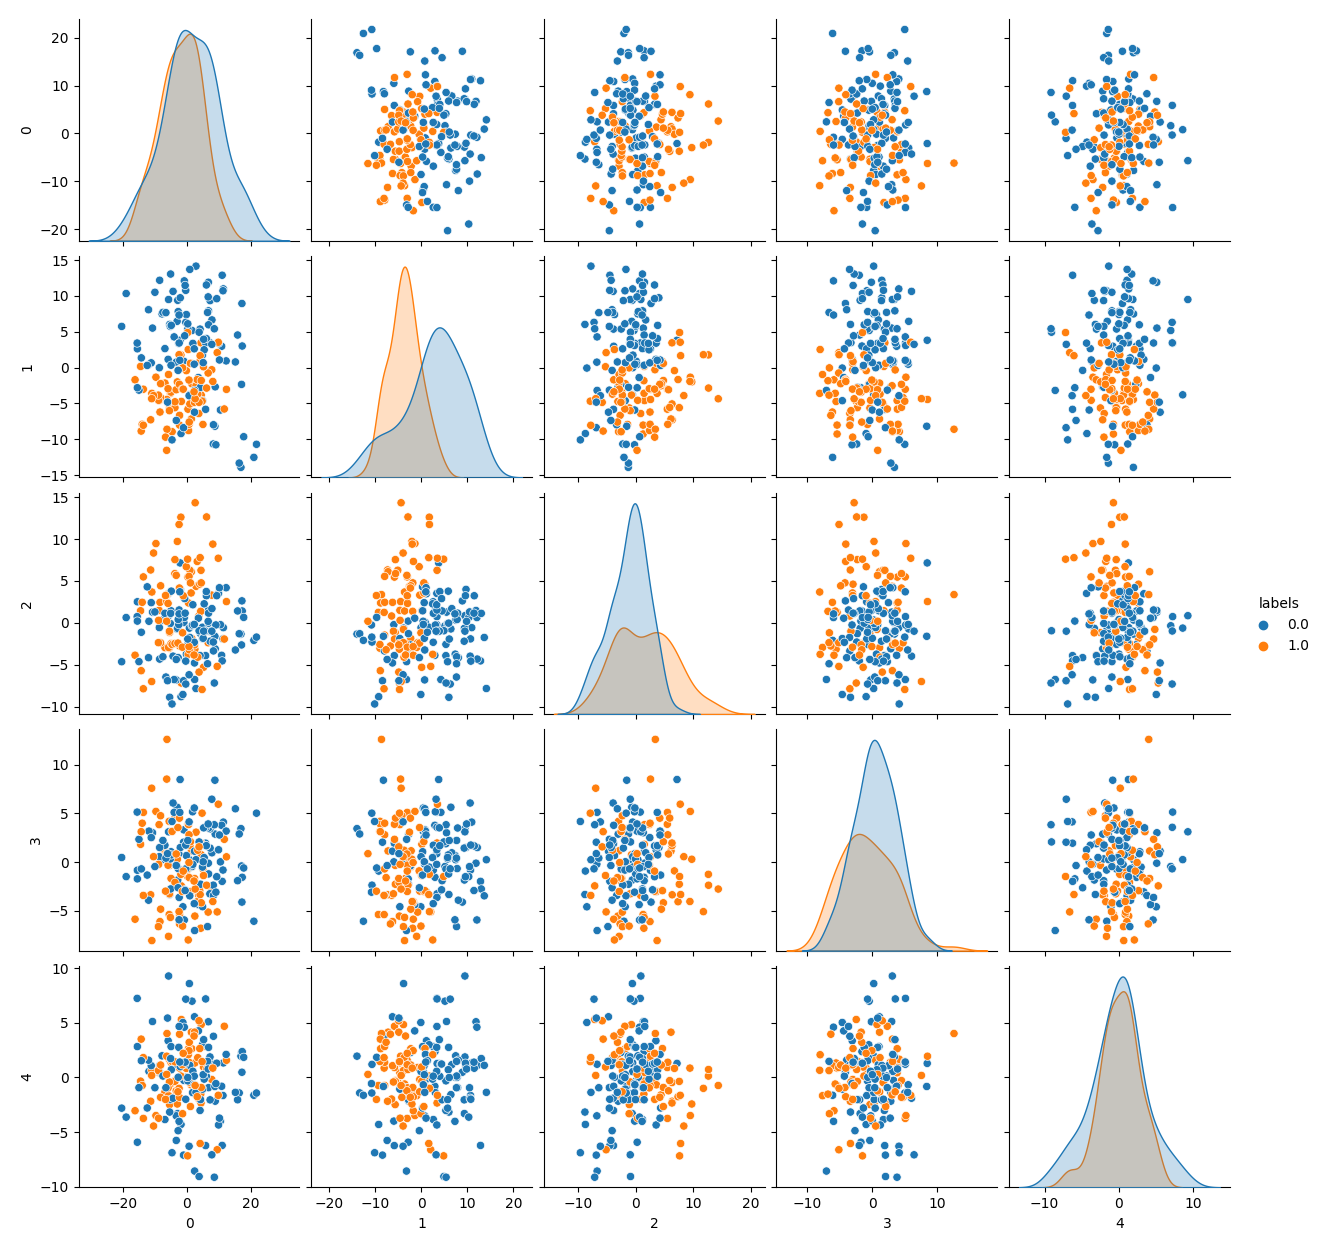
\includegraphics[width=1\linewidth]{1c/True labels sns.png}  
  \caption{Put your sub-caption here}
  \label{fig:sub-first}
\end{subfigure}
\begin{subfigure}{.5\textwidth}
  \centering
  % include second image
  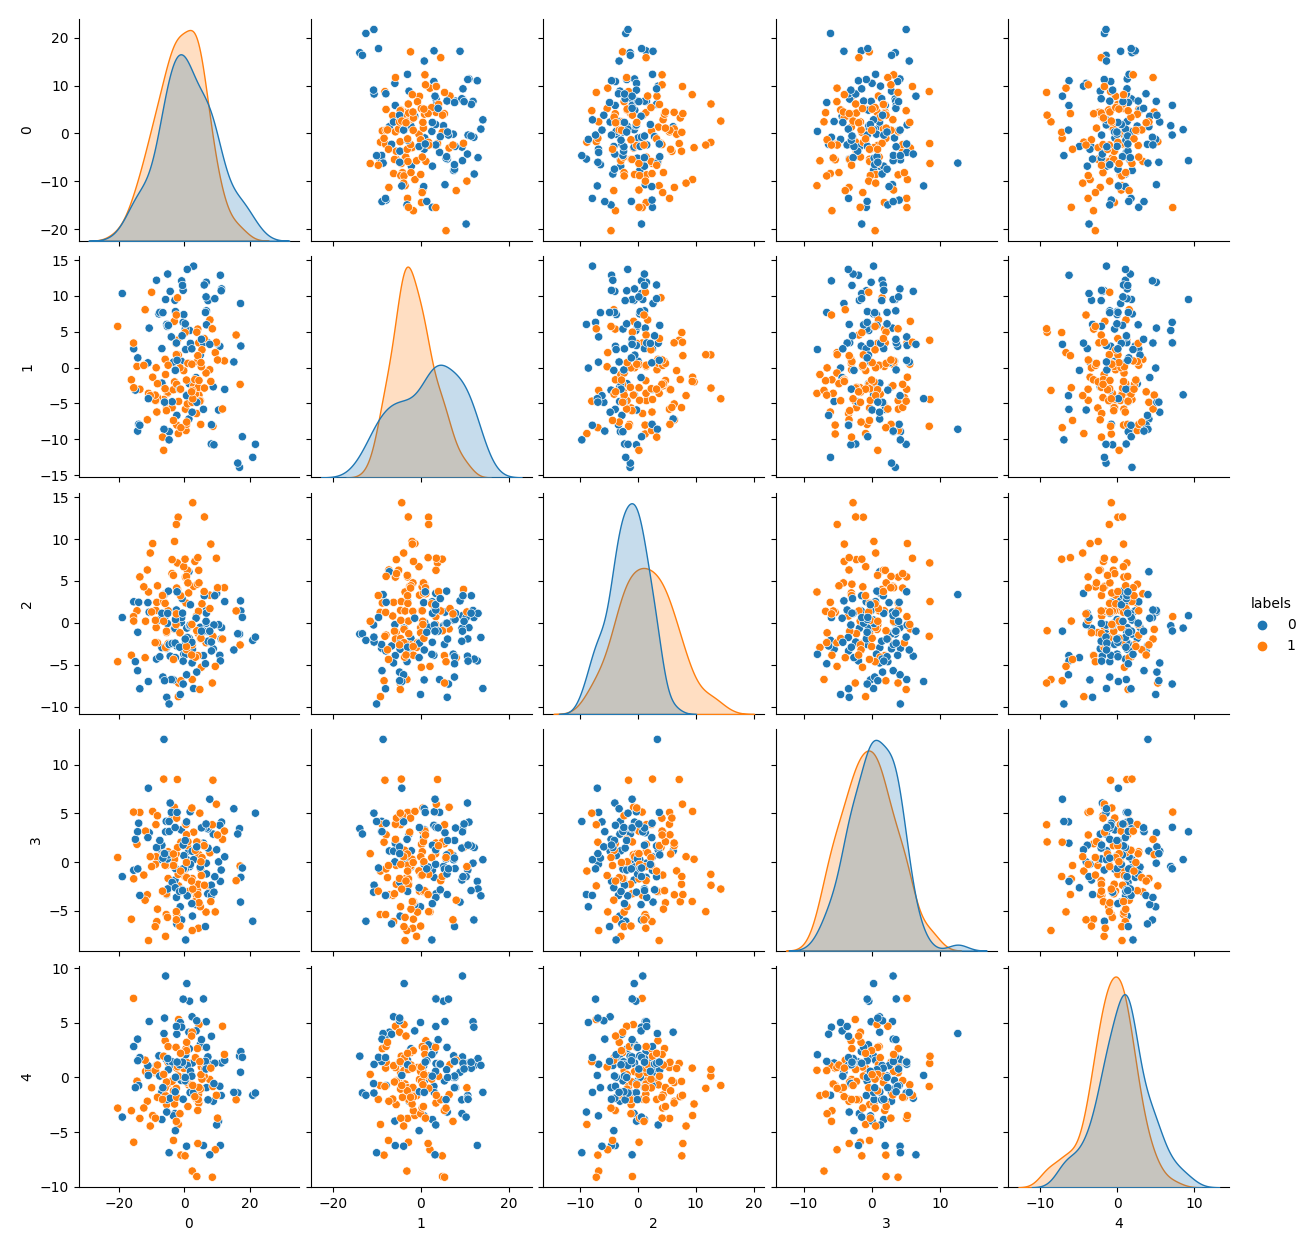
\includegraphics[width=1\linewidth]{1c/two clusters gmm sns.png}  
  \caption{Put your sub-caption here}
  \label{fig:sub-second}
\end{subfigure}
\caption{Put your caption here}
\label{imp pixels}
\end{figure}
\subsection{Discussion}

\end{document}